\chapter{Sentiment Analysis}
People's opinions, feelings and sentiments towards entities such as products, services, other people, events, news, issues, topics, etc., can be in substantial volume, complex and challenging to be understood and processed by machines and computers. Thus, sentiment analysis, also known as opinion mining, started to popularise along with the rise of social media when a large amount of digital text data were suddenly available for mining. Natural language processing (NLP) helps computers process and understand human-based language to perform a repetitive task. Sentiment analysis is a niche of NLP, and it aims at quantifying the positivity, negativity and/or neutrality of implied or expressed in a given text.

Social media have provided large platforms for people to freely share their opinions and express their views on any subject across various geographical and spatial boundaries. They have also allowed people to connect, influence and be influenced by such opinions and views. Management science researchers studied these interactions in the 1940s and 1950s among people in organizations. Since 2002, with social media, those studies have been performed at grand scales with much data. Thus, advanced sentiment analysis research has been performed in political science, economics, finance and management science as they are heavily dependent on public opinions. 

\section{Rule-Based Methods}
Conventional NLP techniques rely on rules to process textual data to extract opinion, polarity, topic, and other information within the data. Tokenization, part-of-speech tagging, lemmatization and removal of stop words are some rules and techniques used to process data prior to analysis. Tokenization is the separation/breaking down of text data into words, and the space between words in a document is commonly used as the delimiter of separation. Consider the example below:
\begin{align}
    \label{POS_example_sent}
    &\text{“The price of Bitcoin wasn’t great today!”}\\
\intertext{Tokenizing the result above results in the list:}
    &\text{['The', 'price', 'of', 'Bitcoin', 'was',  'n’t', 'great', 'today', '!']}
\end{align}
In sentiment analysis, the tokenized sentence would be compared to a predefined list of polarized (positive and negative) words. A naive way to get the polarity of the sentence would be to count the number of positive and negative words in the predefined polarized lists. The limitations are obvious; we are not considering the context in which the words are used nor the preceding words. Part-of-speech tagging refers to the classification of the token in a document based on a predefined assignment. Tokens are classified as adjectives, adverbs, nouns, verbs, etc. (the complete list can be obtained through the \href{https://universaldependencies.org/u/pos/}{Universal POS tags}). POS tagging is used to describe the syntactic structuring of a sentence.
\begin{figure}[H]
    \centering
    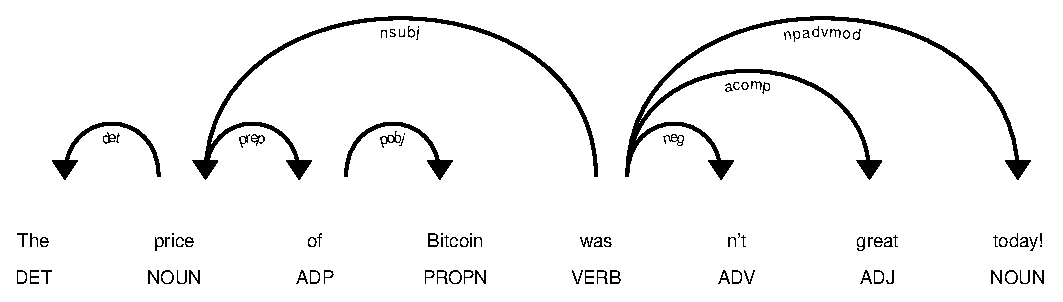
\includegraphics[scale=0.8]{CHAPTER_4/POS_tagging.eps}
    \caption{Part-of-speech tagging of sentence at \refeq{POS_example_sent} using spaCy}
    \label{PSO_EXAMPLE}
  \end{figure}
\noindent Lemmatization refers to the process of reducing words  to their base form, also known as lemma. For example, the words below can be reduced as follows:
\begin{align*}
    &\text{great → good} \\
    &\text{happiness → happy} \\
    &\text{stemming → stem}
\end{align*}
It allows mapping the meaning of multiple words at one time by reducing the former to its base. The assumption is that both forms retain the same meaning syntactically. Moreover, the removal of stop words is often performed to eliminate neutral words or those that bring no additional value within a sentence. Examples of such words would be “the”, “a”, “is”, etc. Since rule-based models are performed individually over each word, the simple removal of stop words reduced the computation time of such models. However, such models are minimal, computationally demanding and often inaccurate. Thus, with the rise of computation power available and machine learning, statistical and embedding-based models were developed to tackle those limitations.
\section{Word Embedding}
Processing raw data from ruled based method is not ideal. A numerical representation of text data would be more appropriate for mathematical models to perform NLP. Word embedding is the representation of text data as vectors in a vector space. Words with similar meanings would be considered very close to each other in such a space. Moreover, from linear algebra, we would expect that normalised vectors of words with similar meanings to be close. Word embedding techniques are categorised among two types: frequency-based embedding and prediction-based embedding. 

Frequency-based embedding refers to the vectorization of words based on the frequency of occurrence of words in a document. The three frequency-based embedding types are Count Vector, TF-IDF (Term Frequency-Inverse Term Frequency) Vector and Co-Occurence Matrix with a fixed context window. Such embedding results in a very sparse vector of high dimensionality which are computationally challenging to manipulate. 

Prediction-based embedding predicts a target word based on the context (neighbouring words). Developed by \cite{Mikolov2013}, the word2vec was introduced. Word2vec is a word embedding method derived from two techniques: CBOW (Continuous Bag of Words) and the Skip-Gram Model. The CBOW attempts to predict the probability of a word in the centre from a given context, while the Skip-Gram model is the opposite of the CBOW model; it tries to predict the context of words given a centre word.
\section{Transformer Model (Attention Mechanism)}
\label{section: transformers}
Attention in neural networks attempts to emulate the human brain's cognitive attention, focusing on the only relevant part of the data while neglecting the rest. Developed by a team at Google Brain in 2017 \cite{Vaswani2017}, transformers are the current state-of-the-art attention techniques (instead of recurrence) for processing contextual data; text, audio, video, speech, etc. Like the RNN, LSTM and GRU, transformers process sequential data as well, with the exception that transforms process all input at once, thus allowing parallelization. Transformers consist of two main parts: the encoder and the decoder. The encoder processes the input document identifies the critical text, and creates an embedding for the text based on the latter's importance to other words in the document. On the other hand, the decoder tries to get the text back from the embedding created by the encoder.
\begin{figure}[H]
    \centering
    \includegraphics[scale=1.1]{CHAPTER_4/c4_fig_transformer_layer_draw.png}
    \caption{Transformer Layer \protect\cite{Vaswani2017}}
    \label{TRANSFORMER_LAYER}
  \end{figure}
  The left part of the architecture is the encoder, while the right side is the decoder. This structure allows the transformer model for parallelization computations instead of sequential (RNN, LSTM and GRU). Transformer models can now solve natural language processing problems with higher accuracy. We introduce two commonly used transformation models: BERT and RoBERTa. 

  Bidirectional Encoder Representations from Transformers (BERT) was developed by Google \cite{Jacob2018}. BERT uses only the encoder part of the transformer, similar to the original transformer in \cite{Vaswani2017}. 
  
  BERT can create word representations that are dynamically influenced by the surrounding words, whereas word2vec has a fixed representation for each word independent of the context in which it occurs. When it was published, it led BERT to achieve multiple state-of-the-art NLP tasks, including sentiment analysis \cite{Chiorrini2021}. Several pre-trained BERT models from the unlabeled text are currently available (due to a large number of data and parameters required for training) and can be re-adapted using transfer learning. 
  
  RoBERTa, the Robustly Optimized BERT Pretaining Approach, was also developed by Google \cite{Yinhan2019}. The approach found that BERT was currently under-trained and could potentially do much better. RoBERTa uses an extensively large amount of hyperparameters, tuning and optimization. Additionally, much more data was also used during training. BERT used 16 Gb of data from CC-news while RoBERTa was trained on 160bg of data from CC-news (92 Gb), OpenWebText (38 Gb), and addition data from Stories (31 Gb) \cite{Yinhan2019}.
